\documentclass[notes,11pt, aspectratio=169]{beamer}

\usepackage{pgfpages}
% These slides also contain speaker notes. You can print just the slides,
% just the notes, or both, depending on the setting below. Comment out the want
% you want.
\setbeameroption{hide notes} % Only slide
%\setbeameroption{show only notes} % Only notes
%\setbeameroption{show notes on second screen=right} % Both

%\usepackage[scaled=1.0]{helvet}
\usepackage{array}


\usepackage{tikz}
\usepackage{verbatim}
\setbeamertemplate{note page}{\pagecolor{gray!5}\insertnote}
\usetikzlibrary{positioning}
\usetikzlibrary{snakes}
\usetikzlibrary{calc}
\usetikzlibrary{arrows}
\usetikzlibrary{decorations.markings}
\usetikzlibrary{shapes.misc}
\usetikzlibrary{matrix,shapes,arrows,fit,tikzmark}
\usepackage{amsmath}
\usepackage{mathpazo}
\usepackage{hyperref}
\usepackage{lipsum}
\usepackage{multimedia}
\usepackage{graphicx}
\usepackage{multirow}
\usepackage{graphicx}
\usepackage{dcolumn}
\usepackage{bbm}
\newcolumntype{d}[0]{D{.}{.}{5}}

\usepackage{changepage}
\usepackage{appendixnumberbeamer}
\newcommand{\beginbackup}{
   \newcounter{framenumbervorappendix}
   \setcounter{framenumbervorappendix}{\value{framenumber}}
   \setbeamertemplate{footline}
   {
     \leavevmode%
     \hline
     box{%
       \begin{beamercolorbox}[wd=\paperwidth,ht=2.25ex,dp=1ex,right]{footlinecolor}%
%         \insertframenumber  \hspace*{2ex} 
       \end{beamercolorbox}}%
     \vskip0pt%
   }
 }
\newcommand{\backupend}{
   \addtocounter{framenumbervorappendix}{-\value{framenumber}}
   \addtocounter{framenumber}{\value{framenumbervorappendix}} 
}


\usepackage{graphicx}
\usepackage[space]{grffile}
\usepackage{booktabs}

% These are my colors -- there are many like them, but these ones are mine.
\definecolor{blue}{RGB}{0,114,178}
\definecolor{red}{RGB}{213,94,0}
\definecolor{yellow}{RGB}{240,228,66}
\definecolor{green}{RGB}{0,158,115}

\hypersetup{
  colorlinks=false,
  linkbordercolor = {white},
  linkcolor = {blue}
}


%% I use a beige off white for my background
\definecolor{MyBackground}{RGB}{255,253,218}

%% Uncomment this if you want to change the background color to something else
%\setbeamercolor{background canvas}{bg=MyBackground}

%% Change the bg color to adjust your transition slide background color!
\newenvironment{transitionframe}{
  \setbeamercolor{background canvas}{bg=white}
  \begin{frame}}{
    \end{frame}
}

\setbeamercolor{frametitle}{fg=blue}
\setbeamercolor{title}{fg=black}
\setbeamertemplate{footline}[frame number]
\setbeamertemplate{navigation symbols}{} 
\setbeamertemplate{itemize items}{-}
\setbeamercolor{itemize item}{fg=blue}
\setbeamercolor{itemize subitem}{fg=blue}
\setbeamercolor{enumerate item}{fg=blue}
\setbeamercolor{enumerate subitem}{fg=blue}
\setbeamercolor{button}{bg=MyBackground,fg=blue,}

%%% TIKZ STUFF
\tikzset{   
	every picture/.style={remember picture,baseline},
	every node/.style={anchor=base,align=center,outer sep=1.5pt},
	every path/.style={thick},
}
\newcommand\marktopleft[1]{%
	\tikz[overlay,remember picture] 
	\node (marker-#1-a) at (-.3em,.3em) {};%
}
\newcommand\markbottomright[2]{%
	\tikz[overlay,remember picture] 
	\node (marker-#1-b) at (0em,0em) {};%
}
\tikzstyle{every picture}+=[remember picture] 
\tikzstyle{mybox} =[draw=black, very thick, rectangle, inner sep=10pt, inner ysep=20pt]
\tikzstyle{fancytitle} =[draw=black,fill=red, text=white]
%%%% END TIKZ STUFF


% If you like road maps, rather than having clutter at the top, have a roadmap show up at the end of each section 
% (and after your introduction)
% Uncomment this is if you want the roadmap!
% \AtBeginSection[]
% {
%    \begin{frame}
%        \frametitle{Roadmap of Talk}
%        \tableofcontents[currentsection]
%    \end{frame}
% }
\setbeamercolor{section in toc}{fg=blue}
\setbeamercolor{subsection in toc}{fg=red}
\setbeamersize{text margin left=1em,text margin right=1em} 

\newenvironment{wideitemize}{\itemize\addtolength{\itemsep}{10pt}}{\enditemize}
\newenvironment{wideenumerate}{\enumerate\addtolength{\itemsep}{10pt}}{\endenumerate}

\usepackage{environ}
\NewEnviron{videoframe}[1]{
  \begin{frame}
    \vspace{-8pt}
    \begin{columns}[onlytextwidth, T] % align columns
      \begin{column}{.58\textwidth}
        \begin{minipage}[t][\textheight][t]
          {\dimexpr\textwidth}
          \vspace{8pt}
          \hspace{4pt} {\Large \sc \textcolor{blue}{#1}}
          \vspace{8pt}
          
          \BODY
        \end{minipage}
      \end{column}%
      \hfill%
      \begin{column}{.42\textwidth}
        \colorbox{green!20}{\begin{minipage}[t][1.2\textheight][t]
            {\dimexpr\textwidth}
            Face goes here
          \end{minipage}}
      \end{column}%
    \end{columns}
  \end{frame}
}

\title[]{\textcolor{blue}{ECN 453: Pricing and Monopoly}}
\author[PGP]{}
\institute[FRBNY]{\small{\begin{tabular}{c c c}
Nicholas Vreugdenhil \\
\end{tabular}}}
\date{} 

\begin{document}

% Title Slide
\begin{frame}
\maketitle
  \centering
\end{frame}

% INTRO

\begin{frame}{Optimal pricing for a monopolist}
\begin{wideitemize}
	\item Today we will discuss \textbf{optimal pricing for a monopolist}.
	\item The `optimal price' is the \textbf{price which maximizes profit}.
	\item Why is this useful?
	\begin{wideitemize}
		\vspace{11pt}
		\item \underline{Policymakers}: understand how the monopolist is reducing welfare (due to its pricing)
		\item \underline{Firm strategy}: Suppose you are working as an economist in a firm that is launching a new product. How should you set prices for this new product to maximize profits?
	\end{wideitemize}
	\item (Most of what we will see today is review from your previous courses)
\end{wideitemize}
\end{frame}

\begin{frame}{Plan}
  \begin{wideenumerate}
  	\item Pricing: example using a table
  	\item Pricing: MR=MC
    \item Pricing: elasticities
    \item Welfare costs of monopoly pricing and regulation
  \end{wideenumerate}
\end{frame}

\begin{frame}{Plan}
  \begin{wideenumerate}
	\item \textbf{Pricing: example using a table}
	\item Pricing: MR=MC
	\item Pricing: elasticities
	\item Welfare costs of monopoly pricing and regulation
\end{wideenumerate}
\end{frame}

\begin{frame}{Pricing: example using a table}
	\begin{wideitemize}
		\item \textbf{Question:} 
		\item You are working as an economist in a firm and you know demand and total cost in the table below for a new product.
		\item How should you set optimal prices (prices that maximize profit)? (In this example you can only sell whole numbers of the product.)
	\end{wideitemize}
	\vspace{11pt}
	\begin{figure}
		\begin{tabular}{|c|c|c|c|c|c|c|}
			\hline
			price& demand  &TR  & MR & TC  & MC & profit  \\
			\hline
			6 & 0 &  &  & 4.5 & & \\
			5 & 1 &   &  & 5  & & \\
			4 & 2 &  &  & 5.5 & & \\
			3 & 3 &  &  & 6 & & \\
			2 & 4 &  &  & 6.5 & & \\
			1 & 5 &  &  & 7 & & \\
			\hline
		\end{tabular}
	\end{figure}
\end{frame}

\begin{frame}{Pricing: example using a table}
	\begin{wideitemize}
		\item \textbf{Question:} 
		\item You are working as an economist in a firm and you know demand and total cost in the table below for a new product.
		\item How should you set optimal prices (prices that maximize profit)? (In this example you can only sell whole numbers of the product.)
	\end{wideitemize}
	\vspace{11pt}
\makebox[\linewidth][c]{
		\begin{tabular}{|c|c|c|c|c|c|c|}
			\hline
			price& demand  &TR  & MR & TC  & MC & profit  \\
			\hline
			6 & 0 &  0&-  & 4.5 & - & -4.5 \\
			5 & 1 & 5  & 5  & 5  & 0.5 &0 \\
			4 & 2 & 8 & 3 & 5.5 &0.5 & 2.5\\
			\marktopleft{a1} 3 & 3 & 9 & 1 & 6 & 0.5& 3 \markbottomright{a1}{red} \\
			2 & 4 & 8 &  -1& 6.5 & 0.5&1.5 \\
			1 & 5 & 5 &  -3& 7 & 0.5& -2\\
			\hline
		\end{tabular}
}
{\tikz[overlay,inner sep=1pt]
\node[draw=red,rounded corners,fit=(marker-a1-a.north west) (marker-a1-b.south east)] {};}
\begin{wideitemize}
	\item \textbf{Idea:} Keep raising prices so long as $MR \geq MC$. 
\end{wideitemize}
\end{frame}

\begin{frame}
  \begin{wideenumerate}
	\item Pricing: example using a table
	\item \textbf{Pricing: MR=MC}
	\item Pricing: elasticities
	\item Welfare costs of monopoly pricing and regulation
\end{wideenumerate}
\end{frame}

\begin{frame}{Pricing: MR=MC}
	\begin{wideitemize}
		\item In the previous example we could only sell whole numbers of the product.
		\item When we can sell fractions of the product (which we usually assume) then the optimal price will occur when:
		\begin{align*}
		 MR = MC
		 \end{align*}
	 	\item This is a \underline{very} important formula.
		\item I will now apply the formula to solve for a monopolist's optimal price.
		\item (This should be a review from your previous courses)
	\end{wideitemize}
\end{frame}

\begin{frame}{Pricing: MR=MC: monopoly example}
	  \begin{wideitemize}
		\item \textbf{Question:}
		\item Suppose a monopolist faces the demand curve $q=2-\frac{1}{5}p$ and has constant marginal cost of 5. What is the optimal price?
		\pause
		\item \textbf{Solution:}
		\item Compute MR from the demand curve using the `double the slope' rule: MR = 10-10q
		\item Next, use MR=MC to find the optimal quantity: 
		\begin{align*}
			\underbrace{10-10q}_{MR} = \underbrace{5}_{MC}
		\end{align*}
		\item Rearranging, get the optimal quantity: $q^*=0.5$.
		\item Finally, plug in $q^*=0.5$ to the demand curve to get the optimal price:
		\begin{align*}
			p^*=10-5 \times 0.5 = 7.5
		\end{align*}
	\end{wideitemize}
\end{frame}

\begin{frame}{Pricing: MR=MC: algorithm}
	\begin{wideitemize}
		\item Lets reiterate those steps again - follow this algorithm to find the optimal price for a monopolist given demand and marginal cost.
	\end{wideitemize}
	\begin{wideenumerate}
		\vspace{11pt}
		\item Get MR from the demand curve. (Use the 'double the slope' trick if demand is linear.)
		\item Use MR=MC; solve for the optimal quantity
		\item Plug the optimal quantity back into the demand curve to get the optimal price
	\end{wideenumerate}
	\begin{wideitemize}
	\vspace{11pt}
		\item I'll now repeat these steps using a graphical analysis.
	\end{wideitemize}
\end{frame}

\begin{frame}{Pricing: MR=MC: graph}
	\begin{figure}
		\begin{tikzpicture}[scale=0.55]
			
			%y axis.....................
			\draw [->] (0,0) to (0,12) node [left] {$price$};
			
			%x axis......................
			\draw [->] (0,0) to (12,0) node [below] {$quantity$};
			
			% D curve...................
			\draw [thick] (0,10)  to  (10,0)  node [above right] {$D$};
			
			% MC=S curve...................
			\draw [thick] (0,1)  to  (12,1)  node [right] {$MC$};
			
		\end{tikzpicture}
	\end{figure}
\end{frame}

\begin{frame}{Pricing: MR=MC: graph 1. get MR from demand}
	\begin{figure}
		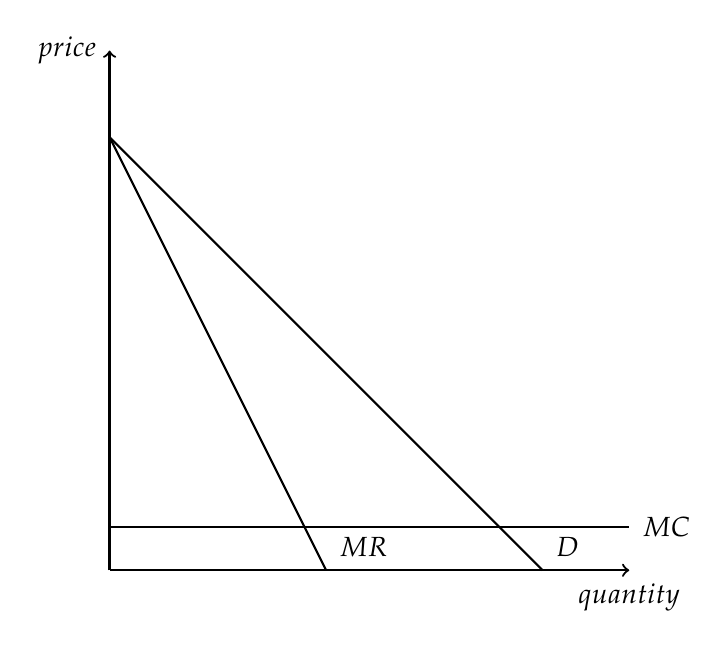
\begin{tikzpicture}[scale=0.55]
			
			%y axis.....................
			\draw [->] (0,0) to (0,12) node [left] {$price$};
			
			%x axis......................
			\draw [->] (0,0) to (12,0) node [below] {$quantity$};
			
			% D curve...................
			\draw [thick] (0,10)  to  (10,0)  node [above right] {$D$};
			
			% MC=S curve...................
			\draw [thick] (0,1)  to  (12,1)  node [right] {$MC$};
			
			% MR curve....................
			\draw [thick] (0,10) to (5,0);
			\node [above right] at (5,0) {$MR$};
			
		\end{tikzpicture}
	\end{figure}
\end{frame}

\begin{frame}{Pricing: MR=MC: 2. Use MR=MC; get $q^*$}
	\begin{figure}
		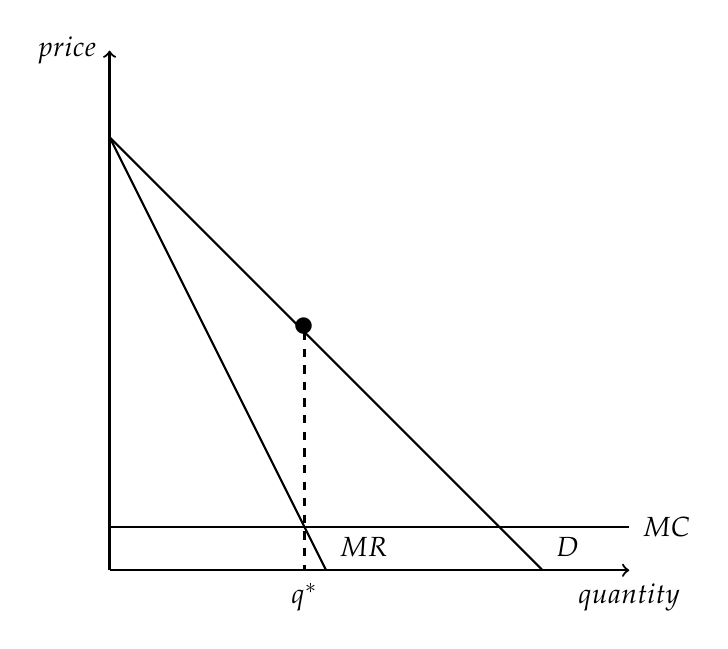
\begin{tikzpicture}[scale=0.55]
			
			%y axis.....................
			\draw [->] (0,0) to (0,12) node [left] {$price$};
			
			%x axis......................
			\draw [->] (0,0) to (12,0) node [below] {$quantity$};
			
			% D curve...................
			\draw [thick] (0,10)  to  (10,0)  node [above right] {$D$};
			
			% MR curve....................
			\draw [thick] (0,10) to (5,0);
			\node [above right] at (5,0) {$MR$};
			
			% MC=S curve...................
			\draw [thick] (0,1)  to  (12,1)  node [right] {$MC$};
			
			% dashed lines to equilibrium.............
			\draw [dashed] (4.5,5.5) to (4.5,0) node [below] {$q^*$};
			
			% equilibrium points.......................
			\node [black] at (4.5,5.25) {\LARGE \textbullet};

			
		\end{tikzpicture}
	\end{figure}
\end{frame}

\begin{frame}{Pricing: MR=MC: 3. Get $p^*$ from the demand curve.}
\begin{figure}
		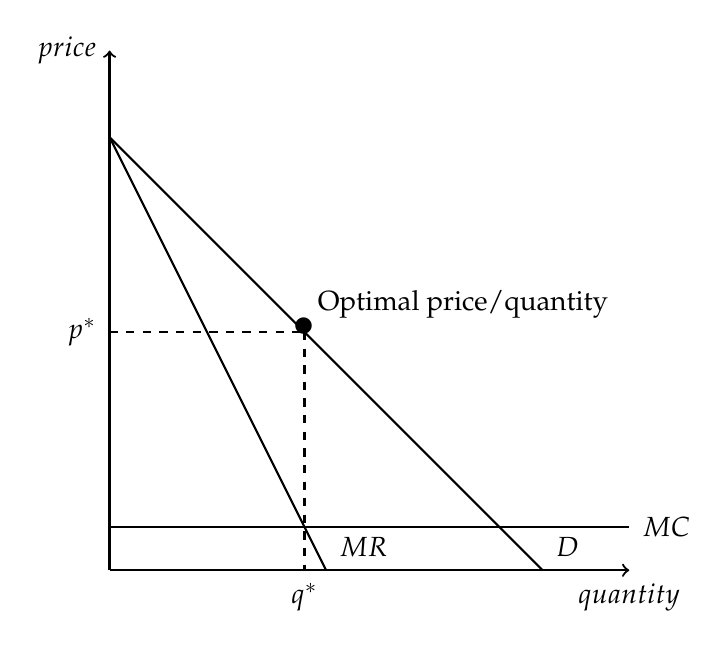
\begin{tikzpicture}[scale=0.55]
		
		%y axis.....................
		\draw [->] (0,0) to (0,12) node [left] {$price$};
		
		%x axis......................
		\draw [->] (0,0) to (12,0) node [below] {$quantity$};
		
		% D curve...................
		\draw [thick] (0,10)  to  (10,0)  node [above right] {$D$};
		
		% MR curve....................
		\draw [thick] (0,10) to (5,0);
		\node [above right] at (5,0) {$MR$};
		
		% MC=S curve...................
		\draw [thick] (0,1)  to  (12,1)  node [right] {$MC$};
		
		% dashed lines to equilibrium.............
		\draw [dashed] (0,5.5) node [left] {$p^*$} to (4.55,5.5); 
		\draw [dashed] (4.5,5.5) to (4.5,0) node [below] {$q^*$};
		
		% equilibrium points.......................
		\node [black] at (4.5,5.25) {\LARGE \textbullet};
		
		% labels..............................
		\node [black, above right] at (4.5,5.5) {Optimal price/quantity};
		
	\end{tikzpicture}
\end{figure}
\end{frame}

\begin{frame}{Plan}
	\begin{wideenumerate}
		\item Pricing: example using a table
		\item Pricing: MR=MC
		\item \textbf{Pricing: elasticities}
		\item Welfare costs of monopoly pricing and regulation
	\end{wideenumerate}
\end{frame}

\begin{frame}{Elasticity rule}
	\begin{wideitemize}
		\item There is a relationship between the optimal price and demand elasticity. 
		\item This is known as the \textbf{elasticity rule}:
		\begin{align*}
			\underbrace{\frac{p-MC}{p}}_{\text{Margin}} = \underbrace{\frac{-1}{\epsilon}}_{\text{Inverse elasticity}}
		\end{align*}
		\item \textbf{Note:} divide by price on the left-hand-side \underline{not} cost.
		\item Equivalently we can isolate the price on the left-hand-side:
		\begin{align*}
			p = \frac{MC}{1 + \frac{1}{\epsilon}}
		\end{align*}
	\end{wideitemize}
\end{frame}

\begin{frame}{Elasticity rule: math (optional)}
	\begin{wideitemize}
		\item The elasticity rule comes from $MR=MC$. Let's unpack the math.
		\pause
		\item If the inverse demand curve is $p=P(q)$ then total revenue is:
		\begin{align*}
			TR = p q = P(q) q
		\end{align*}
		\item Marginal revenue is then (applying the product rule):
		\begin{align*}
			MR = \frac{d TR}{d q} = \frac{d P(q) q}{d q} = p + P'(q) q
		\end{align*}
		\item Now, setting MR = MC:
		\begin{align*}
			p + P'(q) q = MC
		\end{align*}
		\item Rearranging and applying $\epsilon = \frac{dq}{dp} \frac{p}{q}$:
		\begin{align*}
			\frac{p - MC}{p} = -P'(q) \frac{q}{p} = \frac{-1}{\epsilon}
		\end{align*}
	\end{wideitemize}
\end{frame}

\begin{frame}{Elasticity rule: $\frac{p-MC}{p}= \frac{-1}{\epsilon}$ }
	\begin{wideitemize}
		\item Let's check this rule holds for the example where we used $MR=MC$.
		\item Before, we showed that given demand $p=10-5q$ and $MC=5$, the optimal price is $p^*=7.5$ and optimal quantity is $q^*=0.5$.
		\pause
		\begin{wideitemize}
		\vspace{11pt}
		\item Left-hand-side of the elasticity rule is: $\frac{p-MC}{p} = \frac{7.5-5}{7.5} = 1/3$
		\item Right-hand-side of the elasticity rule requires computing the elasticity. First, rearrange demand so that $q=2-\frac{1}{5} p$. Then, the elasticity is:
		\begin{align*}
			\epsilon = \frac{dq}{dp} \frac{p}{q} = -\frac{1}{5} \times \frac{7.5}{0.5} = -3
		\end{align*}
		\item So, right-hand-side $= \frac{-1}{\epsilon} = \frac{-1}{-3} = 1/3 =$ left-hand-side
		\item So, the elasticity rule works!
		\end{wideitemize}
	\end{wideitemize}
\end{frame}

\begin{frame}{Using the elasticity rule}
		\begin{wideitemize}
			\item Why is the elasticity rule a useful way to think about optimal prices?
			\item It turns out it is really useful for real-world empirical applications. Why? \pause
			\begin{wideitemize}
				\vspace{11pt}
				\item For example, suppose you are working as an economist in a firm and you are trying to optimally price a product. 
				\item Typically, you will know the MC. You can (using econometric methods which outside the scope of this course) find the demand elasticity.
				\item Then just plug MC and demand elasticity into the elasticity rule to get the optimal price.
			\end{wideitemize}
		\end{wideitemize}
\end{frame}

\begin{frame}{Plan}
	\begin{wideenumerate}
		\item Pricing: example using a table
		\item Pricing: MR=MC
		\item Pricing: elasticities
		\item \textbf{Welfare costs of monopoly pricing and regulation}
	\end{wideenumerate}
\end{frame}

\begin{frame}{Welfare costs of monopoly pricing}
	\begin{columns}
		\begin{column}{0.5\textwidth}
			\begin{figure}
				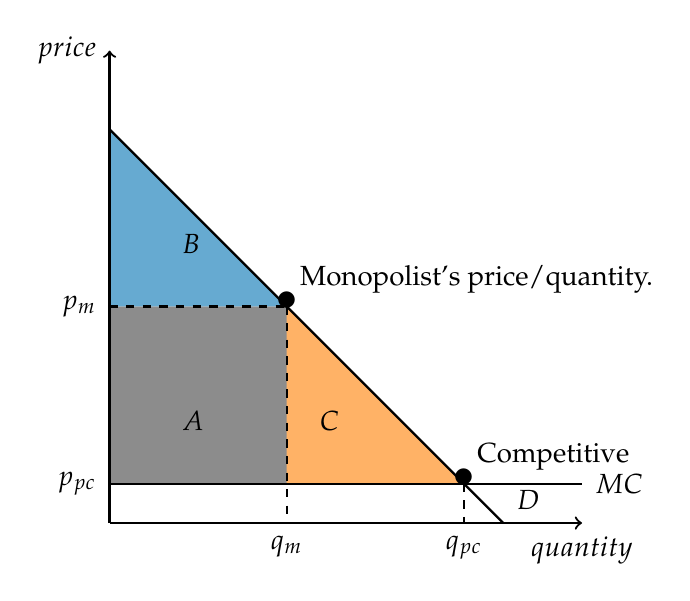
\begin{tikzpicture}[scale=0.5]
					\fill [darkgray!60] (0,1) -- (0,5.5) -- (4.5,5.5) -- (5.5,1) -- cycle;
					\fill [blue!60] (0,5.5) -- (4.5,5.5) -- (0,10) -- cycle;
					\fill [orange!60] (4.5,1) -- (4.5,5.5) -- (9,1) -- cycle;
					
					%y axis.....................
					\draw [->] (0,0) to (0,12) node [left] {$price$};
					
					%x axis......................
					\draw [->] (0,0) to (12,0) node [below] {$quantity$};
					
					% D curve...................
					\draw [thick] (0,10)  to  (10,0)  node [above right] {$D$};
					
					% MR curve....................
					%\draw [thick] (0,10) to (5,0);
					%\node [above right] at (4.5,-0.1) {$MR$};
					
					% MC=S curve...................
					\draw [thick] (0,1)  to  (12,1)  node [right] {$MC$};
					
					% dashed lines to equilibrium.............
					\draw [dashed] (0,5.5) node [left] {$p_m$} to (4.55,5.5); 
					\draw [dashed] (4.5,5.5) to (4.5,0) node [below] {$q_m$};
					
					% dashed lines to new equilibrium.........
					\draw [dashed] (0,1) node [left] {$p_{pc}$} to (9,1); 
					\draw [dashed] (9,1) to (9,0) node [below] {$q_{pc}$};
					
					% equilibrium points.......................
					\node [black] at (4.5,5.25) {\LARGE \textbullet};
					\node [black, above right] at (4.5,5.5) {Monopolist's price/quantity.};
					\node [black, above right] at (9,1) {Competitive};
					\node [black] at (9,0.75) {\LARGE \textbullet};
					
					% labels..............................
					%\node [black, above right] at (4.5,5.5) {Monopolist's price/quantity.};
					\node [above right] at (1.5,6.5) {$B$};
					\node [above right] at (5,2) {$C$};
					\node [above right] at (1.5,2) {$A$};
				\end{tikzpicture}
			\end{figure}
		\end{column}
		\begin{column}{0.5\textwidth} \pause
			\begin{wideitemize}
				\item Here's the diagram from before with the competitive price/quantity (this is where MC=D and is denoted by $q_{pc}, p_{pc}$
				\item Area A: Producer surplus (equal to total profit if fixed costs=0)
				\item Area B: Consumer surplus
				\item Monopoly sets price `too high' and quantity `too low' compared to the competitive case. This causes a dead-weight-loss: Area C
			\end{wideitemize}
		\end{column}
	\end{columns}
\end{frame}

\begin{frame}{Welfare costs of monopoly pricing: summary}
	\begin{wideitemize}
		\item Competition would result in prices that maximize \textbf{total surplus}
		\item Monopolist sets prices `optimally' (i.e. optimal for itself) and maximizes \textbf{profit}
		\item The monopolist ends up setting a price `too high' and a quantity `too low' compared to competition.
		\item The difference in total surplus between a monopolist and competition is called the \textbf{dead-weight-loss}.
		\item Monopoly is an example of a \textbf{market failure}.
	\end{wideitemize}
\end{frame}

\begin{frame}{Regulating monopolies}
	\begin{wideitemize}
		\item How can we correct the market failure of a monopoly and increase total surplus/reduce dead-weight-loss?
		\item One option: break up the monopoly into smaller firms that compete with each other.
		\item This is an example of \textbf{antitrust policy} (policies that correct market failure due to a lack of competition)
	\end{wideitemize}
\end{frame}

\begin{frame}{Regulating monopolies: case study of Facebook vs FTC}
\begin{figure}
	\includegraphics[scale=0.2]{logos.jpeg}
\end{figure}
\begin{wideitemize}
	\item \textbf{Background:}
	\item In 2012 Facebook acquired Instagram
	\item In 2014 Facebook acquired Whatsapp
\end{wideitemize}
\end{frame}

\begin{frame}{Regulating monopolies: case study of Facebook vs FTC}
	\begin{figure}
		\includegraphics[scale=0.15]{ftc.jpeg}
	\end{figure}
	\begin{wideitemize}
		\item In 2020 the Federal Trade Commission (FTC) sued Facebook.
		\item FTC was seeking to (amongst other things) require \textbf{divestiture} (the forced sale) of Whatsapp and Instagram.
		\item FTC alleged ``Facebook has engaged in a systematic strategy [of acquisitions]... to eliminate threats to its monopoly''
		\begin{wideitemize}
			\item FTC: ``Facebook’s actions to entrench and maintain its monopoly deny consumers the benefits of competition.''
		\end{wideitemize}
	\end{wideitemize}
\end{frame}

\begin{frame}{Regulating monopolies: case study of Facebook vs FTC}
	\begin{figure}
		\includegraphics[scale=0.15]{outcome.jpeg}
	\end{figure}
	\begin{wideitemize}
		\item \textbf{Outcome:} Court dismissed the FTC's complaint in June 2021.
		\item Court stated that FTC did not prove that Facebook was a monopoly.
		\item In addition, court argued that FTC waited too long to challenge the acquisitions.
		\item The court allowed Facebook to refile at a future date with more evidence that Facebook is a monopoly.
	\end{wideitemize}
\end{frame}

%\begin{frame}{Regulating monopolies: case study of Facebook vs FTC}
	%\begin{wideitemize}
		%\item About a week ago the FTC refiled with more evidence that Facebook is a monopoly, so the case in ongoing.
		%\item This and other antitrust complaints centered on large tech companies will likely continue in the near future.
	%\end{wideitemize}
%\end{frame}

\begin{frame}{Regulating monopolies: other examples of breaking up a monopoly}
	\begin{wideitemize}
		\item \underline{Standard Oil}: enormous oil company run by John D. Rockefeller.
		\item Standard Oil was broken up into companies including Chevron, ExxonMobil, and Amoco at the start of the 20th century.
		\item \underline{AT\&T}: Broken up into many smaller firms in 1984
		\item There are many other examples of monopoly breakups, as well as attempted breakups (e.g. Microsoft in 2001)
		\item That said, as we will see in Part 3 of the course, much of antitrust policy is focused on \textit{preventing} new monopolies.
	\end{wideitemize}
\end{frame}

\begin{frame}{Regulating monopolies: marginal and average cost pricing}
		\begin{wideitemize}
			\item Sometimes it is not possible to break up the monopoly into smaller firms.
			\begin{wideitemize}
				\vspace{11pt}
				\item Examples: a power plant, a bridge
		   	\end{wideitemize}
			\item These are known as \textbf{`natural monopolies'}
			\item How should we regulate these monopolies?
		\end{wideitemize}
\end{frame}

\begin{frame}{Regulating monopolies: marginal cost pricing}
	\begin{wideitemize}
		\item One possibility for regulation: \textbf{marginal cost pricing}
		\item \textbf{Idea}: force the monopolist to set $p=MC$ 
		\begin{wideitemize}
			\vspace{11pt}
			\item This is the perfect competition price and so there will be no dead-weight-loss.
		\end{wideitemize}
		\item \textbf{But there is an issue.} Suppose that the monopolist has a cost function of $C(q) = F + cq$ where $F$ is a fixed cost and $c$ is the constant marginal cost.
		\pause
		\item Then, the monopolists profit will be:
		\begin{align*}
			Profit = TR-TC = pq - F - cq
		\end{align*}
		\item Since $p=MC=c$, the monopolists profit will be $-F$ i.e. \underline{negative}!
		\item Clearly, this firm would \textbf{shutdown} under regulation because profit is negative. To prevent firm shutdown, a possibility is to also give the firm a \textbf{government subsidy of $F$}.
	\end{wideitemize}
\end{frame}

\begin{frame}{Regulating monopolies: average cost pricing}
	\begin{wideitemize}
		\item Another possibility for regulation: \textbf{average cost pricing}
		\item \textbf{Idea}: force the monopolist to set $p=AC$. This is the price consistent with the monopolist making zero profits:
		\begin{wideitemize}
			\vspace{11pt}
			\item If $Profit = 0$ then, equivalently, $TR=TC$.
			\item Since $TR=pq$, $TR=TC$ is equivalent to $pq=TC$.
			\item Rearranging: $p = TC/q = AC$
		\end{wideitemize}
	\end{wideitemize}
\end{frame}

\begin{frame}{Regulating monopolies: average cost pricing}
	\begin{wideitemize}
		\item Essentially, average cost pricing allows the monopolist to exercise its monopoly power only to cover its fixed costs.
		\begin{wideitemize}
			\vspace{11pt}
			\item So, a government subsidy is no longer necessary.
		\end{wideitemize}
		\item Average cost pricing is commonly used to regulate privately owned power plants in the US and many other countries and in this context it is called `rate of return regulation'.
		\item We will now see average cost pricing on the previous monopoly graph.
	\end{wideitemize}
\end{frame}

\begin{frame}{Regulating monopolies: average cost pricing}
	\begin{figure}
		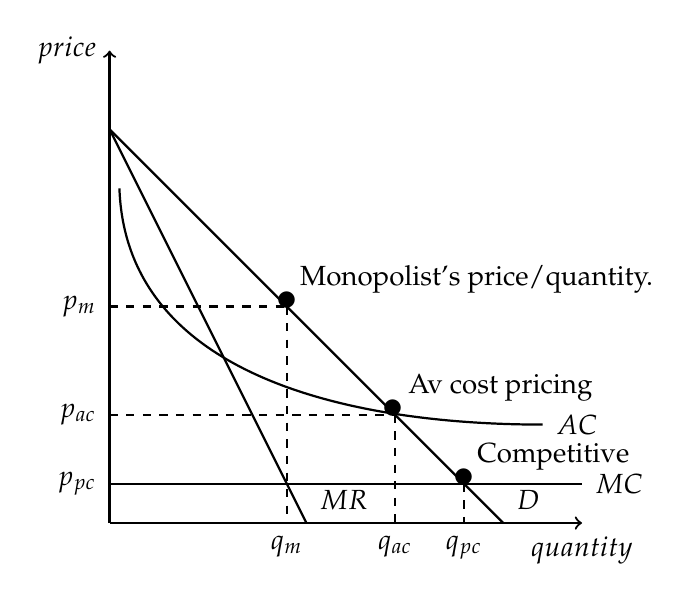
\begin{tikzpicture}[scale=0.5]
			
			%y axis.....................
			\draw [->] (0,0) to (0,12) node [left] {$price$};
			
			%x axis......................
			\draw [->] (0,0) to (12,0) node [below] {$quantity$};
			
			% D curve...................
			\draw [thick] (0,10)  to  (10,0)  node [above right] {$D$};
			
			% MR curve....................
			\draw [thick] (0,10) to (5,0);
			\node [above right] at (5,0) {$MR$};
			
			% MC=S curve...................
			\draw [thick] (0,1)  to  (12,1)  node [right] {$MC$};
			
			% ATC curve...................
			\draw [thick] (0.25,8.5) to [out=-88,in=180]  (11,2.5) node[right] {$AC$};
			
			% dashed lines to equilibrium.............
			\draw [dashed] (0,5.5) node [left] {$p_m$} to (4.55,5.5); 
			\draw [dashed] (4.5,5.5) to (4.5,0) node [below] {$q_m$};
			
			% dashed lines to new equilibrium.........
			\draw [dashed] (0,1) node [left] {$p_{pc}$} to (9,1); 
			\draw [dashed] (9,1) to (9,0) node [below] {$q_{pc}$};
			
			% dashed lines to new equilibrium.........
			\draw [dashed] (0,2.75) node [left] {$p_{ac}$} to (7.25,2.75); 
			\draw [dashed] (7.25,2.75) to (7.25,0) node [below] {$q_{ac}$};
			
			% equilibrium points.......................
			\node [black] at (4.5,5.25) {\LARGE \textbullet};
			\node [black] at (7.2,2.5) {\LARGE \textbullet};
			\node [black] at (9,0.75) {\LARGE \textbullet};
			
			% labels..............................
			\node [black, above right] at (4.5,5.5) {Monopolist's price/quantity.};
			\node [black, above right] at (7.25,2.75) {Av cost pricing};
			\node [black, above right] at (9,1) {Competitive};
		\end{tikzpicture}
	\end{figure}
	\begin{itemize}
		\item Diagram from before with average cost pricing (quantity = $q_{ac}$, price = $p_{ac}$)
	\end{itemize}
\end{frame}

\begin{frame}{Summary of key points*}
	\vspace{11pt}
	\begin{wideitemize}
		\item Know the optimal price occurs at $MR=MC$ (where `optimal price' means the profit maximizing price) 
		\item Know the steps to solve for the monopolist's optimal price and compute the dead-weight-loss, graphically and using math
		\item Know the elasticity rule
		\item Know three potential solutions to monopoly market failure (and how to apply them): 1. divestment 2. marginal cost pricing 3. average cost pricing.
	\end{wideitemize}
	\vspace{30pt}
	*To clarify, all the material in the slides, problem sets, etc is assessable unless stated otherwise, but I hope this summary might be a useful place to start when studying the material.
\end{frame}

\begin{frame}{References}
	\begin{wideitemize}
		\item Monopoly graph based on: \url{https://github.com/EconoTodd/LaTeX_code/blob/master/naturalmonopoly}
	\end{wideitemize}
\end{frame}

\iffalse
\begin{frame}{Average cost pricing: example}
	\begin{wideitemize}
		\item \textbf{Question:} Suppose that demand is given by $q=4-p$ and total cost is given by $C(q)= \frac{5}{4} + q$. 
		\item (a): What is the dead-weight-loss under average cost pricing?
		\item (b): What is the firm's profit under average cost pricing?
		\item (c): What is the dead-weight-loss under monopoly pricing?
		\item (d): What is the firm's profit under monopoly pricing?
	\end{wideitemize}
\end{frame}

\begin{frame}{Average cost pricing: example - solutions}
	\begin{wideitemize}
		\item \textbf{Question:} Suppose that demand is given by $q=4-p$ and total cost is given by $C(q)= \frac{5}{4} + q$. 
		\item (a): What is the dead-weight-loss under average cost pricing?
		\item Answer: 1/8
		\item (b): What is the firm's profit under average cost pricing?
		\item Answer: 0
		\item (c): What is the dead-weight-loss under monopoly pricing?
		\item Answer: 9/8
		\item (d): What is the firm's profit under monopoly pricing?
		\item Answer: 1.0
	\end{wideitemize}
\end{frame}

\begin{frame}{Marginal cost pricing: example}
	\begin{wideitemize}
		\item \textbf{Question:} Suppose that demand is given by $q=4-p$ and total cost is given by $C(q)= \frac{5}{4} + q$. 
		\item (e): What is the subsidy required to prevent firm shutdown under marginal cost pricing?
	\end{wideitemize}
\end{frame}
\fi

\end{document}
